Taskmanager is een applicatie om te zien welke applicaties er draaien, maar ook om het systeem te monitoren op CPU-belasting, geheugen-, disk- en netwerkgebruik.

Via taskmanager kan je configureren welke applicaties er opgestart worden, je kan niet reagerende applicaties afsluiten en je kan gebruikerssessies beheren.

Om Taskmanager te openen:
\begin{itemize}
\item Klik op het zoek icoon en zoek op Taskmanager
\item Gebruik ctrl+shift+esc
\end{itemize}

\begin{minipage}[t]{\linewidth}
\raggedright
\adjustbox{valign=t}{%
	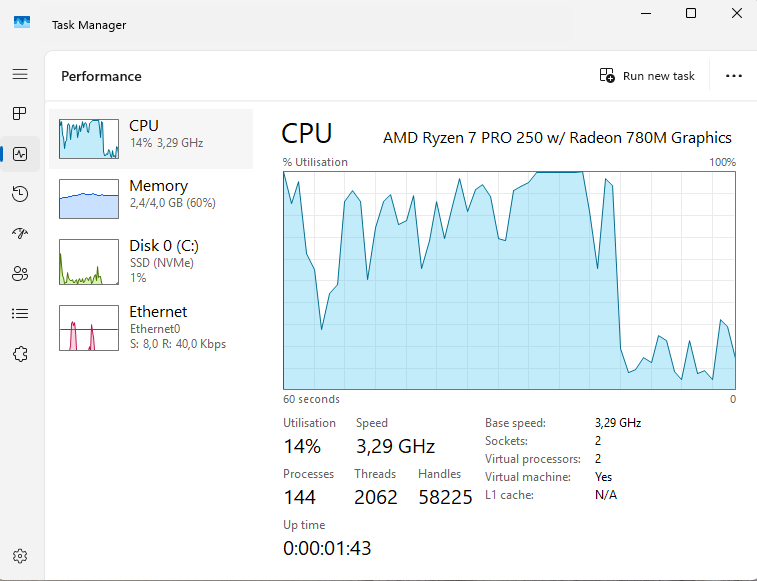
\includegraphics[width=0.99\linewidth]{taskmanager.png}%
}
\end{minipage}

